\documentclass[12pt]{article}
\usepackage[backend=biber]{biblatex}
\addbibresource{ProjectProp.bib}

\usepackage{graphicx} %intersting images
\usepackage{float} %for placement of images
\usepackage{lipsum} %fill
\usepackage{tocloft} %for dots on table of contents
\renewcommand{\cftsecleader}{\cftdotfill{\cftdotsep}}

\begin{document}

\begin{titlepage}
	\centering{
\includegraphics[scale=0.7]{ProjectPropFigure/BUlogo.jpg}\\
	\vspace{3em}
	\bfseries{\large{Department of Electrical and Computer Engineering}}\\
	\vspace{2em}
	\bfseries{\large{Senior Capstone Project Proposal}}\\
	\vspace{2em}
	\bfseries{\Large{Charge Pump}}\\
	\vspace{2em}
	\bfseries{\large{Authors: Derek Brissey \& John Clapham}}\\
	\textit{\large{Advisors: Dr. Brian Huggins \& Dr. Prasad Shastry}}\\
	\vspace{2em}
	\today
	}
\end{titlepage}

	\pagenumbering{roman}

	\begin{abstract}
Radio frequency~(RF) energy harvesting devices can be a useful battery alternative for low power applications such as periodic sensor measurements. A passive charge pump topology using Schottky diodes and capacitors can be implemented to step up the voltage of a low power RF input signal to a usable Direct Current~(DC) steady state. This capstone project will include research and simulation, design, and eventually populating a printed circuit board~(PCB) with specified components for testing. This project will explore how the variabilities in a charge pump design (such as number of stages, capacitor values, and a switching device) can be evaluated to produce a more efficient RF-DC conversion for specified frequencies. The exploration of this design will be conducted in frequencies less than 100kHz for analysis in the time domain with the hope to scale up to RF frequencies.
	\end{abstract}
	
	\newpage
	\tableofcontents
	\newpage
	
	\pagenumbering{arabic}
	
\section{Introduction}
Electromagnetic signals that oscillate in the range of 300MHz to 300GHz are known as Radio Frequency~(RF) waves. Due to the widespread use of RF signals, interest in harvesting the low transmitted energy has become a popular concept. This is known as RF energy harvesting. It is normally difficult to collect enough energy from these RF signals to be usable due to the low input power to the energy harvester. Research suggests a charge pump topology could be used in an energy harvesting system to raise low power RF signals to a usable steady state Direct Current~(DC) voltage level. There are many applications for implementing an energy harvesting device that absorbs high frequency energy signals (from sources such as cell phone towers, radio towers, wireless transmitters, etc.) and outputs a DC signal. These applications include: replacement for small battery low power devices, periodic sensor measurements, remote sensing devices, and more. Figure~\ref{fig:energyharvestsystem} shows a typical energy harvesting system.

\begin{figure}[H]
\centering{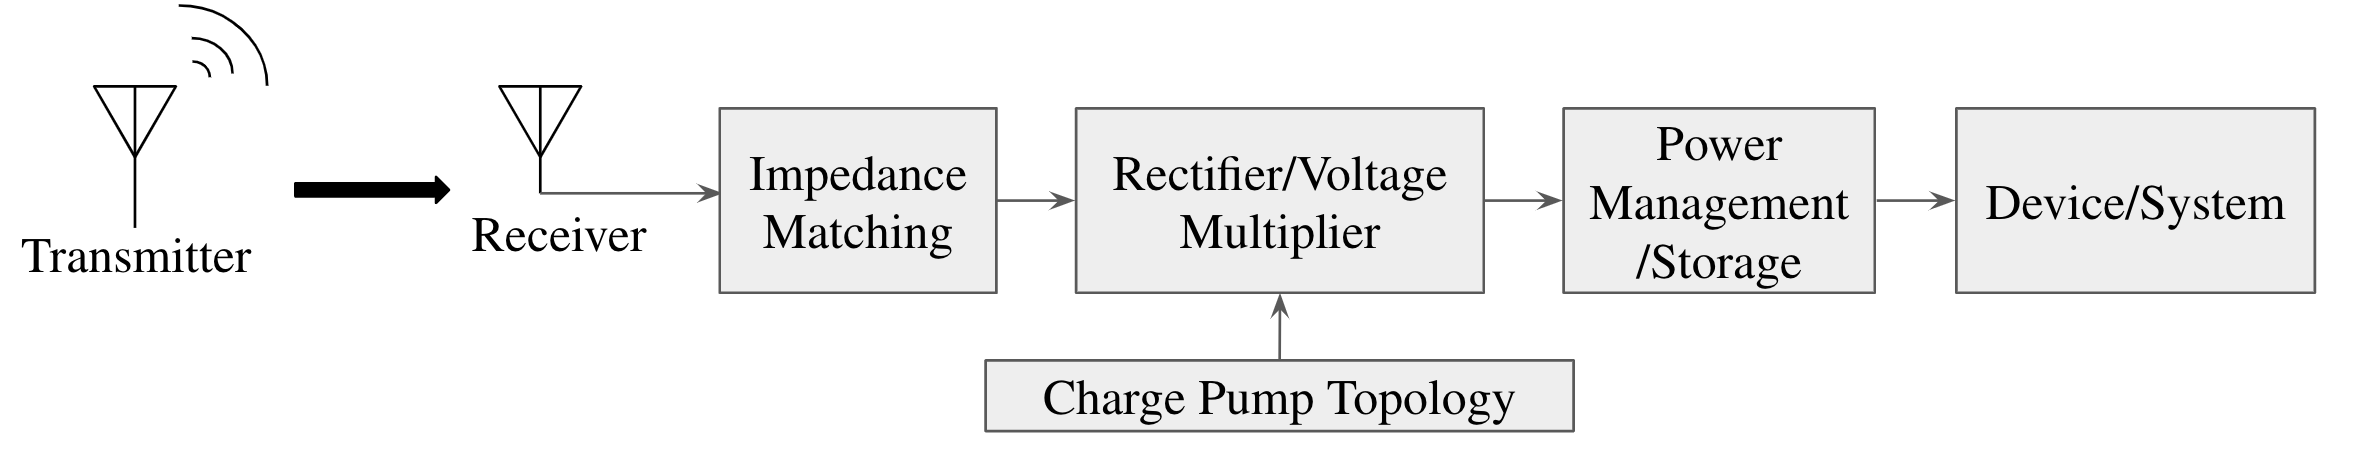
\includegraphics[scale=0.3]{ProjectPropFigure/EnergyHarvestSystem.png}}
\caption{Typical Energy Harvesting System}
\label{fig:energyharvestsystem}
\end{figure}

\noindent A full energy harvesting system starts at the transmitted RF signal generation which is then picked up by a receiver. Then some sort of impedance matching is done to deliver maximum power to the rectifier/voltage multiplier portion of the system. Eventually the power is delivered to a power management or storage system, which is used by the device or system. This project will be looking specifically at how the charge pump topology can be applied to the rectifier/voltage multiplier portion of the system. 

\subsection{Dickson Charge Pump}
In order to use energy harvesting methods as a power supply, the harvested signal needs to be boosted to a higher voltage level through a rectifier or voltage multiplier. This is because the harvested RF signal power is often insufficient to generate the necessary DC voltage level to drive a chip or sensor. The Dickson charge pump is a popular choice for low power wireless systems due to its capability of voltage multiplication. An example of the Dickson charge pump topology is depicted in Figure~\ref{fig:DicksonCP}.
	
\begin{figure}[H]
\centering{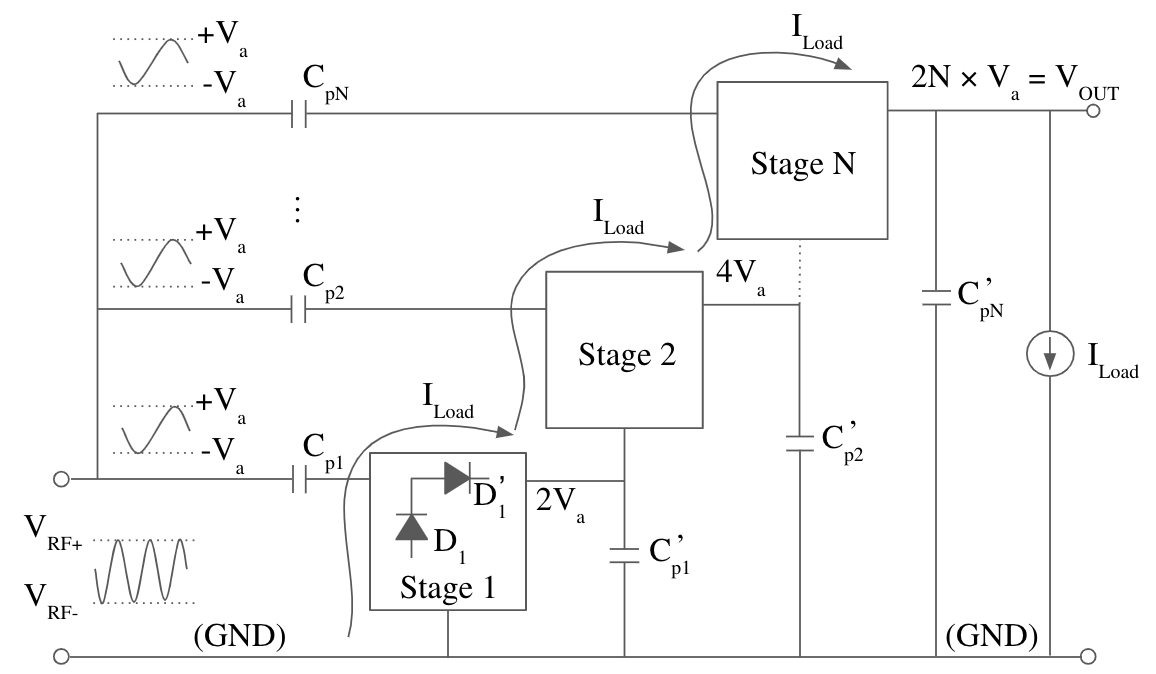
\includegraphics[scale=0.5]{ProjectPropFigure/DicksonBlock.png}}
\caption{Dickson Charge Pump \cite{Guler}}
\label{fig:DicksonCP}
\end{figure}

\noindent The basis of the working charge pump is the switching device. Figure~\ref{fig:DicksonCP} shows diodes in each stage as a passive switching device. The positive half-cycle of the signal will charge capacitors $C^{'}_{pn}$, when the negative half-cycle is reached the capacitors $C^{'}_{pn}$ are unable to discharge due to the diode orientation. As the negative half-cycle of the signal is reached, the capacitors $C_{pn}$ are charged and are unable to discharge on the positive half-cycle of the signal due to the diode orientation. Because the cascading capacitors are being utilized as storage elements a charge is accumulated in the load capacitor, however, the accumulation has diminishing returns and eventually reaches a steady state DC voltage level.\\

\subsection{Problem Statement}
There are many research papers which exist to optimize the performance of the charge pump design, however, little research exists that analyzes the performance of the charge pump for the purpose of RF energy harvesting. The low power RF signal being received at the input of the rectifier/voltage multiplier is difficult to transmit to a usable voltage DC level. This leads to problems with the practicality of RF-DC energy harvesting. It is necessary to create an accurate model of the charge pump for RF applications for an optimal RF-DC conversion.

\section{Project Description}
Charge pumps have been originally designed for use at low frequencies, however, research suggests the charge pump topology can be designed for use in the RF range to eventually be used in an energy harvester system. Although a full energy harvester system has multiple designed components, the focus of this project will be towards the voltage/rectifier portion of the system. A closer look at the full system that will be examined in this project is shown in Figure~\ref{fig:HighLevel}.
	
\begin{figure}[H]
\centering{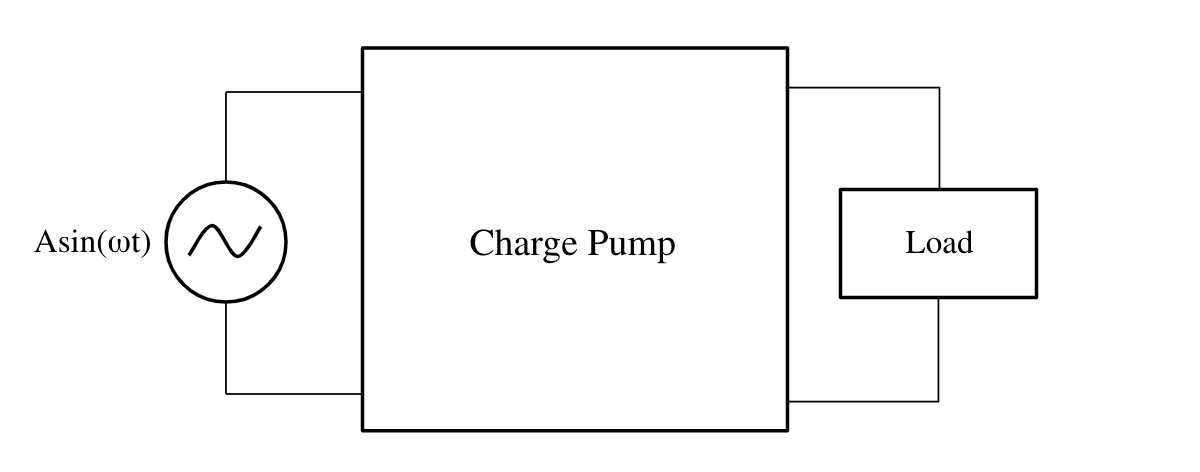
\includegraphics[scale=0.5]{ProjectPropFigure/HighLevelBlock.png}}
\caption{High Level Block Diagram}
\label{fig:HighLevel}
\end{figure}
	
\noindent A sinusoidal signal will be input directly into the charge pump block from a signal generator. The signal will then be converted to a DC voltage and dumped into a load. The signal frequency that will be used will be less than 100kHz in order to perform analysis in the time domain with the hope of scaling up to RF. \\

\noindent All RF-DC charge pumps use capacitors as storage elements in stages and many attempts to optimize the selection of components used for the charge pump have been made. Design criteria for selecting capacitor values, number of stages, and diodes in order to optimize the performance of the charge pump in the RF range is the goal of this project. Multiple papers exist documenting the progress that has been made in RF-DC devices, however, further investigation is needed for improving the efficiency of power conversion, as well as possible circuit topologies, and device implementations. 
	
	\section{Review of Design}
	The DC output of the Dickson charge pump is obtained by the capacitors cyclically charging and discharging depending on the state of the diodes. Several characteristics must be considered when designing a charge pump circuit. The Dickson charge pump will be initially simulated with arbitrarily chosen parameters such as number of stages and capacitor values. Due to the low turn on voltage of Schottky diodes, they are a necessary choice in passive charge pump designs. A Schottky diode will be chosen based off of a low threshold voltage. Other switches such as various transistors have been used, however, research suggests transistors are a better option for charge pump integrated circuit design. A variety of charge pump topologies will be explored. Various signal frequencies will be input to the system with different amplitudes to determine effects on output.

	\section{Project Plan}
	The purpose of this project is to research the affecting parameters of the charge pump and determine possible design criteria. The project will result in providing research for more effective topologies and components used to produce a steady state DC output. The four main stages of the project will include research, simulation, design, and implementation on a PCB. While the idea is to convert RF frequencies~(greater than 500MHz) to DC, experimentally less than 1~kHz will be used to analyze the circuit in the time domain through simulations and laboratory measurements. Then, testing of the design criteria will be scaled up to RF. The functional requirements for the project are listed below:\\
	
\noindent{Functional Requirements}
\begin{itemize}
	\item Explore different charge pump designs and switch components
	\item Develop charge pump design criteria
	\item Convert RF energy to a maximized steady state DC energy
	\item Design and print circuit board for testing purposes
\end{itemize}
	
	\subsection{Research}
	Research papers exploring different energy harvesting devices that include block diagrams, functional designs, power efficiency equations, and suggested design criteria equations have been acquired. Research will be used to analyze various applications of the charge pump for energy harvesting systems as well as for equations to aid in the evaluation of the performance of design.\\
	
	\noindent Three notable research papers have been found:
	\begin{itemize}
	\item ``Applicability of Dickson Charge Pump in Energy Harvesting Systems: Experimental Validation of Energy Harvesting Charge Pump Model" \cite{Vinco}
	\item ``E-WEHP: A Batteryless Embedded Sensor-Platform Wirelessly Powered From Ambient Digital-TV Signals" \cite{Vyas}
	\item ``Power Management in Wireless Power-Sipping Devices: A Survey” \cite{Guler}
	\end{itemize} 
	\vspace{0.5em}

	\noindent Although it has been noticed that these papers base charge pump models from the application of ideal diodes, these research papers will provide a basis for a clear understanding of the task at hand. It could be worth while to instead explore the use of practical diodes to develop charge pump design criteria. Other research papers that will prove useful to the development of the RF-DC charge pump have been listed in the \textit{Bibliography} section on page~\pageref{bibliography}.\\
	
	\noindent Two equations have been found as a possible evaluation of performance of the designed charge pump. Depending on the topology that is being constructed the components can change to increase the Power Conversion Efficiency~(PCE). PCE is the ratio of DC power delivered to the load, to the AC power delivered to the input. The voltage conversion efficiency (VCE) is the ratio between the peak voltage available at the input of the device and the DC voltage available at the output. The VCE and PCE equations that have been found are described as follows~\cite{Guler}:

\begin{equation}
PCE = \frac{P_{Out}}{P_{In}} = \frac{P_{Out}}{P_{Out} + P_{In}}\label{eq:PCE}
\end{equation}
\vspace{1em}

\begin{equation}
VCE = \frac{DC Output Voltage}{RF Peak Voltage} = \frac{V_{Out}}{V_{P}}\label{eq:VCE}
\end{equation}

	\noindent The PCE and VCE equations can be used to compare the efficiency variability in the different designs that will be simulated. PCE and VCE can be optimized by carefully selecting the parts used in the charge pump. It has been suggested that lower levels of reverse leakage in the switching device improve the PCE and VCE of the circuit.\\
	
	\noindent Equations 3 \cite{Vyas}, 4 \cite{Guler}, and 5 \cite{Vinco} are developed equations of the expected steady state DC voltage level across the load capacitor, each from different research papers. Although there are similarities in these equations, there are clear differences that need further investigation. The output voltage equations are as follows:
	
\begin{equation}
V_{out} = 2\times N\times V_{in} - (2\times N + 1)\times V_{th}
\end{equation}

\begin{equation}
V_{out} = (V_{in} - V_{th})(\frac{C_p}{C_{par}})\times N - \frac{I_{LOAD}N}{C_pf}
\end{equation}

\begin{equation}
V_{out} = (N + 1)(V_{in} - V_{th})
\end{equation}

	\noindent Two other notable equations have been suggested for determining the number of stages and capacitor values of the charge pump \cite{Vinco}. These equations are worth mentioning because although the equations could have potential problems due to the basis of ideal diodes, the equations could be a starting point for developing design criteria for the charge pump.

\begin{equation}
N = 2(\frac{V_O}{V_{in}-V_{th}}-1)
\end{equation}

\begin{equation}
C > \frac{N}{fF(N+1)^2R_{EH}}
\end{equation}

	\subsection{Design/Simulation}
	Simulations of the charge pump will be done using ORCAD PSpice. The simulation process will start by performing analysis on various diodes in order to obtain an understanding of the threshold voltage. A low threshold voltage is required for efficient RF-DC conversion. Initial design will be based on the standard Dickson charge pump with 1uF capacitors and Schottky diodes. The input signal will start at 1kHz and the results will be gathered in the time domain.\\
	
	\noindent Analysis will begin with the one stage charge pump. The response and various topologies will be created for analysis consisting of different numbers of stages, and different capacitor values. Stages will continue to be added until a five stage charge pump is created. The time domain response will be recorded from all designs, and then be compared. The most effective design with the best PCE and VCE values~(equations~\ref{eq:PCE}~and~\ref{eq:VCE} on page~\pageref{eq:PCE}) will be selected from the designs. After selecting the design the values of the capacitors will be varied. Simulations will be run in the time domain to analyze the effect of varying values. Next, different topologies will be explored to see if the design can be further improved. A high level block diagram of the system that will be used for evaulation has been shown in Figure~\ref{fig:HighLevel} on page~\pageref{fig:HighLevel}.\\

\noindent The high level block diagram shows the overarching system of that will be used. Only the charge pump, a sinusoidal input, and a load are necessary to represent the system. The underlying charge pump block can be varied through different suggested topologies. Figure~\ref{fig:DicksonCP}  on page~\pageref{fig:DicksonCP} shows the circuit topology that will be used for a majority of the simulation and design stages. The simulation and design stages will continue hand-in-hand throughout the length of the project.

	\subsection{Implementation}
	Once the simulations have been completed, a board design can be created for testing purposes. Prototyping will be done using breadboards and components in the lab. Once verified, a board will be designed and sent to an outside board printing company. The PCB will then be populated with components selected to our specification for testing purposes.
	
	\section{Analysis and Simulation: Current Progress}
	
	The analysis and simulation that has been completed is described in the following sections. Further investigation into optimal design is necessary and will be continued throughout the project.
	
	\subsection{Diode Analysis}
Analysis of the Bat68 diode voltage VS current simulation was completed to find the threshold voltage. A DC sweep has been performed with a step voltage of 1mV in order to compare the threshold voltage listed on the data sheet. The simulation design is shown in Figure~\ref{fig:Bat68} with the output of the DC sweep shown in Figure~\ref{fig:Bat68sim}. The simulation results compare to the data sheet values of the Bat68's typical threshold voltage of 318mV. These simulations are likely to be repeated to determine the diode with the lowest turn on voltage within a reasonable price range.

\begin{figure}[H]
\centering{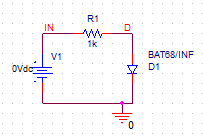
\includegraphics[scale=0.7]{ProjectPropFigure/Bat68.png}}
\caption{Bat68 Diode Analysis Model}
\label{fig:Bat68}
\end{figure}

\begin{figure}[H]
\centering{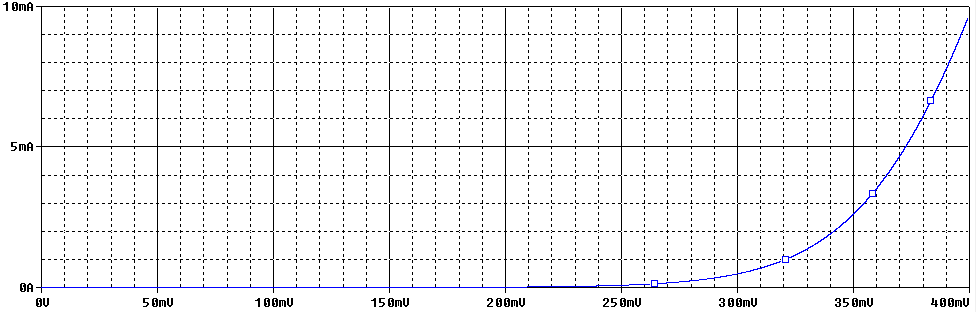
\includegraphics[scale=0.45]{ProjectPropFigure/Bat68sim.png}}
\caption{Bat68 Diode Threshold Voltage}
\label{fig:Bat68sim}
\end{figure}

	\subsection{2-Stage Charge Pump}

\noindent Simulations of a two stage Dickson charge pump with an input amplitude of 1V with a frequency of 1kHz have been completed as a proof of concept. Components were selected to best reflect the physical components available to build a prototype. Standard 0.1uF capacitors and BAT68 diodes were selected to emulate the standard capacitor values and Schottky diodes provided to build the circuit. Figure~\ref{fig:2SCP NSR} shows the layout of the designed charge pump. Time domain responses were plotted showing the voltage stepping up to a steady state. The results were recorded for 50ms. Figures~\ref{fig:2SCP NSR} and~\ref{fig:2SCP NSR Out} show the layout of the designed charge pump and the output voltage across the load capacitor respectively.
	
\begin{figure}[H]
\centering{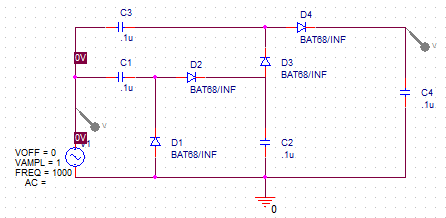
\includegraphics[scale=0.7]{ProjectPropFigure/2stageCPmodel.png}}
\caption{2-Stage Charge Pump}
\label{fig:2SCP NSR}
\end{figure}

\begin{figure}[H]
\centering{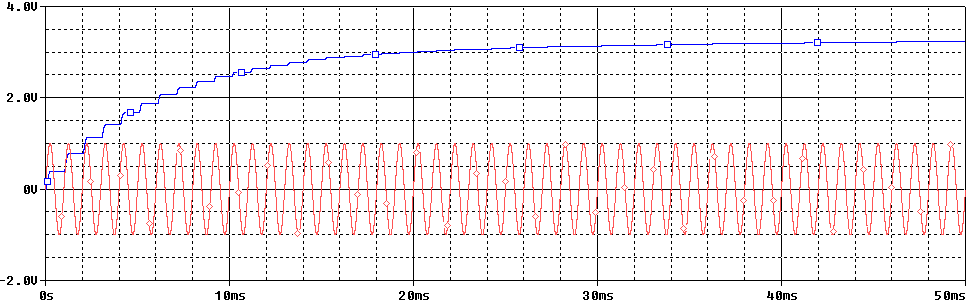
\includegraphics[scale=0.45]{ProjectPropFigure/2stageCPsim.png}}
\caption{2-Stage Charge Pump Output Voltage}
\label{fig:2SCP NSR Out}
\end{figure}

\noindent The voltage across the load capacitor (shown in blue) builds up to a steady state DC voltage level of about 3.25V in 30 cycles of the input frequency (shown in red). \\

\noindent A 50 Ohm resistor was then added as a source resistance to reflect the response of a practical circuit as shown in Figure~\ref{fig:2SCP SR}. The time domain responses of the voltage was taken of the circuit and compared to the response of the circuit without the source resistance. The Simulation was run for 50ms as shown in Figure~\ref{fig:2SCP SR Out} and was compared to simulation shown in Figure~\ref{fig:2SCP NSR Out}.

\begin{figure}[H]
\centering{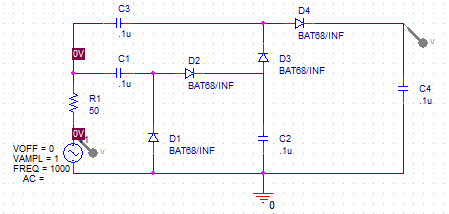
\includegraphics[scale=0.7]{ProjectPropFigure/2stageCPRmodel.png}}
\caption{2-Stage Charge Pump (With Source Resistance)}
\label{fig:2SCP SR}
\end{figure}

\begin{figure}[H]
\centering{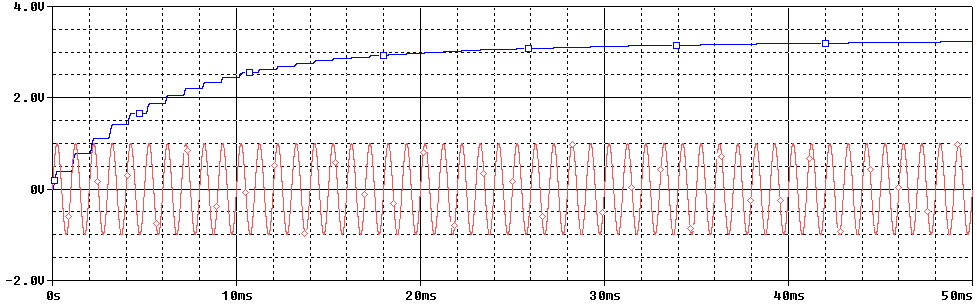
\includegraphics[scale=0.45]{ProjectPropFigure/2stageCPRsim.png}}
\caption{2-Stage Charge Pump Output Voltage (With Source Resistance)}
\label{fig:2SCP SR Out}
\end{figure}

\noindent It is clear that there are no obvious changes to the voltage level output across the load capacitor (shown in blue). The voltage across the load capacitor build up to about 3.25V in about 30 cycles of the input signal (shown in red) again. This means the source resistor can be left out for the rest of the simulations.

\subsection{5-Stage Charge Pump}

A 5-stage charge pump was then simulated in order to see the difference in voltage build up across the load capacitor. The 5-stage charge pump was constructed with similar 0.1uF storage capacitors and the same BAT68 Schottky diodes. The only variability in design was the number of stages. This can be seen in Figure~\ref{fig:5SCPModel}. The input signal has a similar frequency of 1kHz with a 1V amplitude. The input frequency and voltage build up across the load capacitor is shown in Figure~\ref{fig:5SCPSim}.

\begin{figure}[H]
\centering{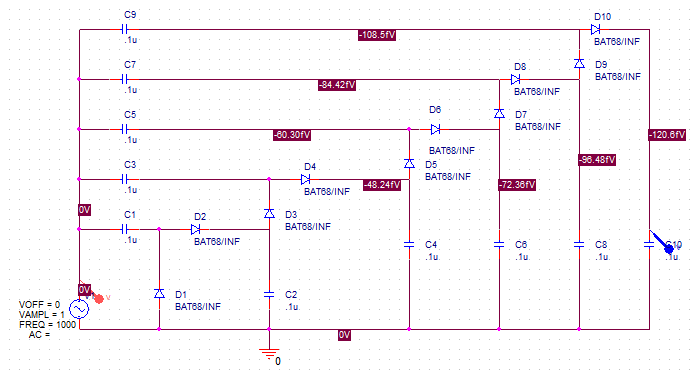
\includegraphics[scale=0.6]{ProjectPropFigure/5stageCPmodel.png}}
\caption{5-Stage Charge Pump}
\label{fig:5SCPModel}
\end{figure}

\begin{figure}[H]
\centering{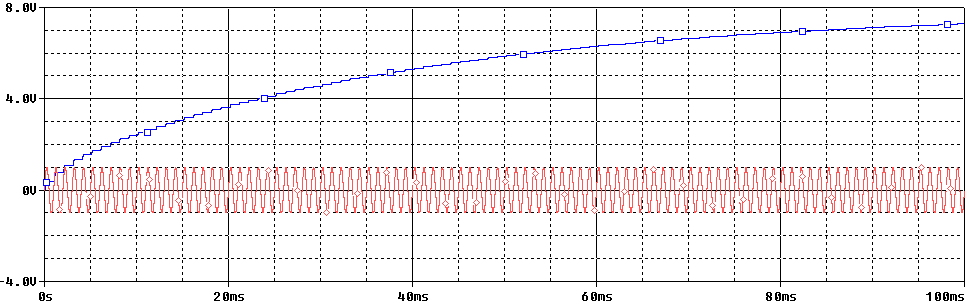
\includegraphics[scale=0.45]{ProjectPropFigure/5stageCPsim.png}}
\caption{5-Stage Charge Pump Output Voltage}
\label{fig:5SCPSim}
\end{figure}

The steady state DC voltage level in the load capacitor (shown in blue) that is reached is about 7V after 100 cycles of the input signal (shown in red).

\subsection{Laboratory Implementation}

\noindent A physical circuit of the 2-stage charge pump has been constructed on a breadboard to measure the response in real time. The physical circuit was built with 0.1uF capacitors similar to the simulations and Schottky diodes 1N5817 were provided by the labs and used. The voltage build up across the load capacitor was captured using burst mode on a signal generator and visually shown on an oscilloscope. Figure~\ref{fig:2SCPLabOut} shows the captured time domain response.

\begin{figure}[H]
\centering{\includegraphics[scale=0.6]{ProjectPropFigure/2stageCPLab_1kHZ_1V.png}}
\caption{2-Stage Charge Pump Lab Output}
\label{fig:2SCPLabOut}
\end{figure}

\noindent The input signal (shown in light blue) was set to a frequency of 1kHz with an amplitude of 1V. This was done to compare lab testing results with the simulations that were done in Pspice. The voltage across the load capacitor (shown in dark blue) charges up to 1.88V in only 10 cycles. This is significantly lower than what was shown in the simulations. Possible reasons that this might be occurring includes factors such as: different threshold voltage, losses in physical circuit not modeled in Pspice, tolerance differences in components, and more. Further investigation is required as to why this is happening.\\

\noindent The same physical circuit was then tested with a lower amplitude of 0.5V. This was done to compare the results of the low input power that would exist in a full energy harvesting system with the results that were gathered in Figure~\ref{fig:2SCPLabOut}. The output was again captured and can be seen ing Figure~\ref{fig:2SCPLabOut2}.

\begin{figure}[H]
\centering{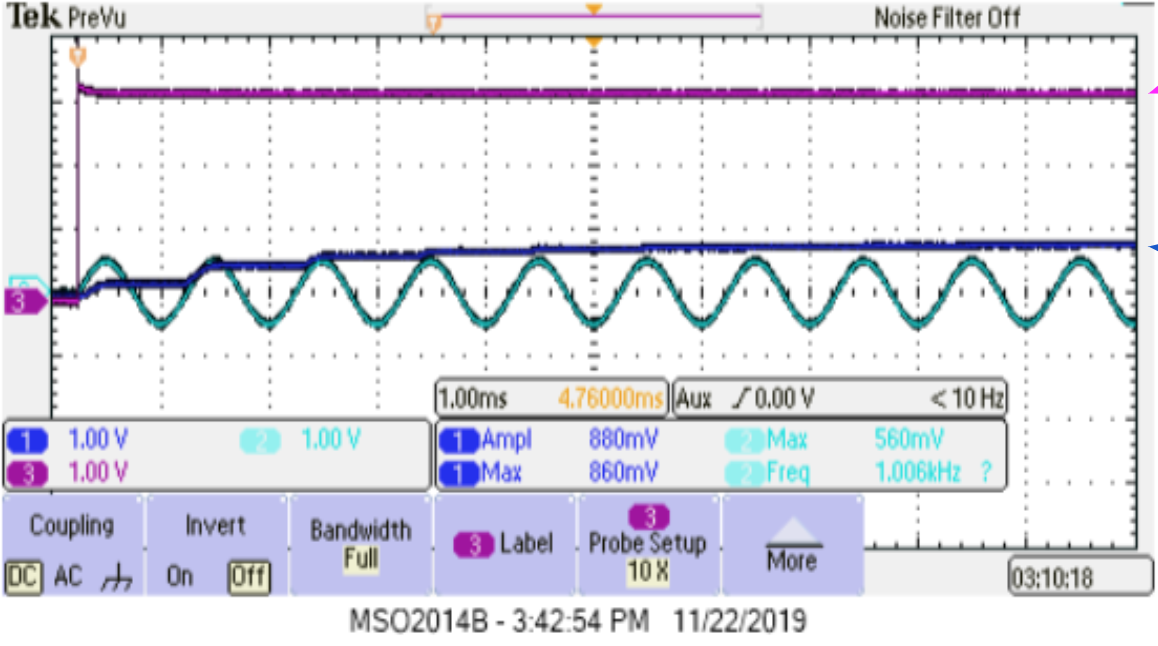
\includegraphics[scale=0.6]{ProjectPropFigure/2stageCPLab_1kHz_500mV.png}}
\caption{2-Stage Charge Pump Lab Output}
\label{fig:2SCPLabOut2}
\end{figure}

Again, the input signal (shown in light blue) is was set to a frequency of 1kHz. The voltage across the load capacitor (shown in dark blue) charges up to a measured 880mV in 10 cycles.

	\subsection{Future Plans}
More simulations must be performed in an effort to optimize the construction of the charge pump. Tests will be performed by varying the different number of levels in the charge pump versus the value of the capacitors to verify which causes a charge pump to charge faster. An attempt to find a correlation or formulate an equation that will optimize the values of capacitors and number of levels for a charge pump will be made using the results of the simulations and physical circuit tests. The PCB will then be constructed according to the design criteria. Parts to construct a PCB will need to be ordered at a later date when a method for optimization is formulated. Further testing will then be completed on the PCB.
	
	\section{Conclusion}
Future uses for RF-DC energy harvesting devices include any low power applications such as period measurement systems, medical sensors, space and aerospace applications, etc. The experience gained from this capstone project will transfer into hardware design and RF design. After designing and implementing to a physical circuit board a better understanding of the design process will be an important outcome. The hope is to have a published research paper at the end of the project that will guide others in the design of a charge pump RF-DC energy harvesting system.
	
	\newpage
	\label{bibliography}
	\nocite{*}
	\printbibliography
	
\end{document}